%%%%%%%%%%%%%%%%%%%%%%%%%%%%%%%%%%%%%%%%%%%%%%%%%%%%%%%%%%
%%%%%%%%%%%%%%%%%%%%%%%%%%%%%%%%%%%%%%%%%%%%%%%%%%%%%%%%%%
%%          Written by Nicolas Bigaouette               %%
%%                    Fall 2012                         %%
%%              nbigaouette@gmail.com                   %%
%%%%%%%%%%%%%%%%%%%%%%%%%%%%%%%%%%%%%%%%%%%%%%%%%%%%%%%%%%
%%%%%%%%%%%%%%%%%%%%%%%%%%%%%%%%%%%%%%%%%%%%%%%%%%%%%%%%%%

\newcommand{\Title}{Full Thesis Title}
\newcommand{\Author}{Nicolas Bigaouette}

% University of Ottawa thesis formatting
\documentclass[author={\Author},title={\Title},draft=true]{uottawa}


%%%%%%%%%%%%%%%%%%%%%%%%%%%%%%%%%%%%%%%%%%%%%%%%%%%%%%%
% Useful macros
%%%%%%%%%%%%%%%%%%%%%%%%%%%%%%%%%%%%%%%%%%%%%%%%%%%%%%%
%%%%%%%%%%%%%%%%%%%%%%%%%%%%%%%%%%%%%%%%%%%%%%%%%%%%%%%%%%%%%%%%%%%%%%%%%%%%%%%%%%%%%%
%%%%%%%%%%%%%%%%%%%%%%%%%%%%%%%%%%%%%%%%%%%%%%%%%%%%%%%%%%%%%%%%%%%%%%%%%%%%%%%%%%%%%%
%%                             Usefull macros                                       %%
%%                           Nicolas Bigaouette                                     %%
%%                          nbigaouette@gmail.com                                   %%
%%%%%%%%%%%%%%%%%%%%%%%%%%%%%%%%%%%%%%%%%%%%%%%%%%%%%%%%%%%%%%%%%%%%%%%%%%%%%%%%%%%%%%
%%%%%%%%%%%%%%%%%%%%%%%%%%%%%%%%%%%%%%%%%%%%%%%%%%%%%%%%%%%%%%%%%%%%%%%%%%%%%%%%%%%%%%

% Needed for \onehalf
% WARNING: This package breaks flushright!!!
% \usepackage{ltugcomn}
% Needed for bold Greek letters
\usepackage{bm}

\newcommand{\mailto}[1]{\href{mailto:#1}{#1}}

\newcommand{\angstrom}{{\AA}ngstr\"om}

% \newcommand{\vecnabla}{\vec{\nabla}}
\newcommand{\vecnabla}{\bm{\nabla}}
\newcommand{\laplacien}[1]{\vecnabla^2 #1}           % Laplacien
\newcommand{\laplacian}[1]{\laplacien{#1}}           % Laplacien
\newcommand{\laplacient}[1]{\vecnabla_{\bot}^{2} #1} % Laplacien transverse
\newcommand{\gradient}[1]{\vecnabla #1}              % Gradient
\newcommand{\grad}[1]{\vecnabla #1}                  % Gradient
\newcommand{\divergence}[1]{\vecnabla \cdot #1}      % Divergence
\newcommand{\rotationnel}[1]{\vecnabla \times #1}    % Rotationnel

% \newcommand{\spherical}{\ensuremath{\mathcal{Y}}_{l,m}\pa{\theta,\phi}}
%                                                     % Spherical Harmonics Y_lm
\newcommand{\spherical}{Y_{l,m}\pa{\theta,\phi}}         % Spherical Harmonics Y_lm
\newcommand{\sphericalp}{Y_{l,m}\pa{\theta',\phi'}}      % Spherical Harmonics Y_lm
\newcommand{\sphericallmp}{Y_{l',m'}\pa{\theta,\phi}}    % Spherical Harmonics Y_lm
\newcommand{\sphericalpc}{Y_{l,m}^*\pa{\theta',\phi'}}   % Spherical Harmonics Y_lm
\newcommand{\sphericalc}{Y_{l,m}^*\pa{\theta,\phi}}      % Spherical Harmonics Y_lm
\newcommand{\gspherical}{\ensuremath{\mathcal{Y}}_{j,l,m}\pa{\theta,\phi}}
                                                         % Genralized Spherical Harmonics
                                                         % Y_jml

\newcommand{\onehalf}{\sfrac{1}{2}}
\newcommand{\onethird}{\sfrac{1}{3}}
\newcommand{\onefourth}{\sfrac{1}{4}}
\newcommand{\twothird}{\sfrac{2}{3}}
\newcommand{\threehalf}{\sfrac{3}{2}}
\newcommand{\fivehalf}{\sfrac{5}{2}}
\newcommand{\eighthalf}{\sfrac{8}{2}}
\newcommand{\summation}[2]{\sum\limits_{#1}^{#2}}

\newcommand{\im}{\textrm{i}}                                    % i = sqrt{-1}

\newcommand{\mum}{\mu \textrm{m}}                               % mu m

\newcommand{\hbartwo}{\frac{\hbar}{2}}
\newcommand{\twohbar}{\frac{2}{\hbar}}

% See:
% http://tex.stackexchange.com/questions/18298/prevent-line-breaking-in-inline-mat
% h-but-allow-flexible-spacing
\newcommand{\preventlinebreak}[1]{{}$\kern-2\mathsurround${}
  \binoppenalty10000 \relpenalty10000 #1{}$\kern-2\mathsurround${}}
\newcommand{\ten}[2]{\preventlinebreak{#1\times10^{#2}}}

\newcommand{\dd}[1]{~\textrm{d} #1}

\newcommand{\del}{\partial}                                     % del

\newcommand{\delexp}[3]{\frac{\del^{#3} #1}{\del #2^{#3}}}          % del^? ? / del?
\newcommand{\dexp}[3]{\frac{\textrm{d}^{#3} #1}{\textrm{d} #2^{#3}}}% d^? ? / d?

\newcommand{\delx}[1]{\delexp{#1}{x}{{}}}                     % del ? / delx
\newcommand{\dely}[1]{\delexp{#1}{y}{{}}}                     % del ? / dely
\newcommand{\delz}[1]{\delexp{#1}{z}{{}}}                     % del ? / delz
\newcommand{\delr}[1]{\delexp{#1}{r}{{}}}                     % del ? / delr
\newcommand{\delt}[1]{\delexp{#1}{t}{{}}}                     % del ? / delt
\newcommand{\deli}[2]{\delexp{#1}{{#2}}{{}}}                  % del ? / del?

\newcommand{\delxs}[1]{\delexp{{#1}}{x}{2}}                     % del^2 ? / delx^2
\newcommand{\delys}[1]{\delexp{{#1}}{y}{2}}                     % del^2 ? / dely^2
\newcommand{\delzs}[1]{\delexp{{#1}}{z}{2}}                     % del^2 ? / delz^2
\newcommand{\delts}[1]{\delexp{{#1}}{t}{2}}                     % del^2 ? / delt^2
\newcommand{\delrs}[1]{\delexp{{#1}}{r}{2}}                     % del^2 ? / delr^2
\newcommand{\delis}[2]{\delexp{{#1}}{#2}{2}}                    % del^2 ? / del?^2

\newcommand{\delxt}[1]{\delexp{{#1}}{x}{3}}                     % del^3 ? / delx^3
\newcommand{\delyt}[1]{\delexp{{#1}}{y}{3}}                     % del^3 ? / dely^3
\newcommand{\delzt}[1]{\delexp{{#1}}{z}{3}}                     % del^3 ? / delz^3
\newcommand{\deltt}[1]{\delexp{{#1}}{t}{3}}                     % del^3 ? / delt^3
\newcommand{\delrt}[1]{\delexp{{#1}}{r}{3}}                     % del^3 ? / delr^3
\newcommand{\delit}[2]{\delexp{{#1}}{#2}{3}}                    % del^3 ? / del?^3

\newcommand{\delxf}[1]{\delexp{{#1}}{x}{4}}                     % del^4 ? / delx^4
\newcommand{\delyf}[1]{\delexp{{#1}}{y}{4}}                     % del^4 ? / dely^4
\newcommand{\delzf}[1]{\delexp{{#1}}{z}{4}}                     % del^4 ? / delz^4
\newcommand{\deltf}[1]{\delexp{{#1}}{t}{4}}                     % del^4 ? / delt^4
\newcommand{\delrf}[1]{\delexp{{#1}}{r}{4}}                     % del^4 ? / delr^4
\newcommand{\delif}[2]{\delexp{{#1}}{#2}{4}}                    % del^4 ? / del?^4

\newcommand{\dx}[1]{\dexp{{#1}}{x}{{}}}                       % d ? / dx
\newcommand{\dy}[1]{\dexp{{#1}}{y}{{}}}                       % d ? / dy
\newcommand{\dz}[1]{\dexp{{#1}}{z}{{}}}                       % d ? / dz
\newcommand{\dt}[1]{\dexp{{#1}}{t}{{}}}                       % d ? / dt
\newcommand{\dr}[1]{\dexp{{#1}}{r}{{}}}                       % d ? / dr
\newcommand{\di}[2]{\dexp{{#1}}{#2}{{}}}                      % d ? / d?

\newcommand{\dxs}[1]{\dexp{{#1}}{x}{{2}}}                     % d^2 ? / dx^2
\newcommand{\dys}[1]{\dexp{{#1}}{y}{{2}}}                     % d^2 ? / dy^2
\newcommand{\dzs}[1]{\dexp{{#1}}{z}{{2}}}                     % d^2 ? / dz^2
\newcommand{\drs}[1]{\dexp{{#1}}{t}{{2}}}                     % d^2 ? / dr^2
\newcommand{\dts}[1]{\dexp{{#1}}{r}{{2}}}                     % d^2 ? / dt^2
\newcommand{\dis}[2]{\dexp{{#1}}{#2}{{2}}}                    % d^2 ? / d?^2

\newcommand{\dtreal}[1]{\frac{\textrm{d} #1}{\textrm{d} t}}         % d ? / dt
\newcommand{\dtsreal}[1]{\frac{\textrm{d}^2 #1}{\textrm{d}t^2}}     % d^2 ? / dt^2
% \newcommand{\dt}[1]{\dot{#1}}                                   % d ? / dt
% \newcommand{\dts}[1]{\ddot{#1}}                                 % d^2 ? / dt^2

\newcommand{\erf}[1]{~\textrm{erf} \left\{#1\right\}}                      % erf{?}
\newcommand{\ex}[1]{\exp{ \left\{ #1 \right\}}}                 % exp{?}
\newcommand{\ep}[1]{\textrm{e}^{\left( #1 \right) }}            % e^(?)
\newcommand{\e}[1]{\textrm{e}^{#1}}                             % e^?
\newcommand{\lnp}[1]{\textrm{ln} \left( #1 \right)}            % ln(?)
\newcommand{\logp}[1]{\textrm{log} \left( #1 \right)}          % log(?)

\newcommand{\cosinus}[1]{\cos #1 }                              % cos
\newcommand{\cosine}[1]{\cosinus{#1}}                           % cos
\newcommand{\sinus}[1]{\sin #1 }                                % sin
\newcommand{\sine}[1]{\sinus{#1}}                               % sin
\newcommand{\cosp}[1]{\cos \left( #1 \right)}                   % cos()
\newcommand{\sinp}[1]{\sin \left( #1 \right)}                   % sin()
\newcommand{\tanp}[1]{\tan \left( #1 \right)}                   % tan()
\newcommand{\sintheta}{\sin \theta}                             % sin theta
\newcommand{\costheta}{\cos \theta}                             % cos theta
\newcommand{\sinptheta}{\sinp{ \theta }}                        % sin(theta)
\newcommand{\cosptheta}{\cosp{ \theta}}                         % cos(theta)
\newcommand{\sinec}[1]{\textrm{ sinc} \left( #1 \right)}        % sinc()
\newcommand{\sinecsquared}[1]{\textrm{ sinc}^2 \left( #1 \right)} % sinc^2()
\newcommand{\cossquared}[1]{\cos^2 \left( #1 \right)}           % cos^2()
\newcommand{\sinsquared}[1]{\sin^2 \left( #1 \right)}           % sin^2()
\newcommand{\tansquared}[1]{\tan^2 \left( #1 \right)}           % tan^2()
\newcommand{\acos}[1]{\textrm{acos} \left( #1 \right)}          % acos()
\newcommand{\asin}[1]{\textrm{asin} \left( #1 \right)}          % asin()
\newcommand{\atan}[1]{\textrm{atan} \left( #1 \right)}          % atan()
\newcommand{\sech}[1]{\textrm{sech} \left( #1 \right)}          % sech()
\newcommand{\tanhyp}[1]{\textrm{tanh} \left( #1 \right)}          % tanh()
\newcommand{\sechsquared}[1]{\textrm{sech}^2 \left( #1 \right)} % sech^2()

\newcommand{\thetatwo}{\frac{\theta}{2}}
\newcommand{\betatwo}{\beta/2}

\newcommand{\dix}[1]{\times 10^{#1}}                            % ? x 10^?

\newcommand{\dint}[1]{~\textrm{d}#1}

\newcommand{\eps}{\epsilon}
\newcommand{\epsz}{\epsilon_0}
\newcommand{\epsr}{\epsilon_r}
\newcommand{\muz}{\mu_0}
\newcommand{\om}{\omega}
\newcommand{\omi}[1]{\omega_{#1}}
\newcommand{\omegaz}{\omega_0}
\newcommand{\omegasquared}{\omega^2}
\newcommand{\omegazsquared}{\omega_0^2}
\newcommand{\omegazsquaredomegasquared}{\omegazsquared - \omegasquared}

% \newcommand{\ve}[1]{\vec{#1}}
\newcommand{\ve}[1]{\textbf{#1}}
\newcommand{\vE}{\ve{E}}
\newcommand{\vA}{\ve{A}}
\newcommand{\vB}{\ve{B}}
\newcommand{\vC}{\ve{C}}
\newcommand{\vD}{\ve{D}}
\newcommand{\vF}{\ve{F}}
\newcommand{\vH}{\ve{H}}
\newcommand{\vJ}{\ve{J}}
\newcommand{\vL}{\ve{L}}
\newcommand{\vM}{\ve{M}}
\newcommand{\vP}{\ve{P}}
\newcommand{\vR}{\ve{R}}
\newcommand{\vS}{\ve{S}}
\newcommand{\vU}{\ve{U}}
\newcommand{\va}{\ve{a}}
\newcommand{\vb}{\ve{b}}
\newcommand{\vc}{\ve{c}}
\newcommand{\vd}{\ve{d}}
\renewcommand{\vee}{\ve{e}}
\newcommand{\vf}{\ve{f}}
\newcommand{\vg}{\ve{g}}
\newcommand{\vh}{\ve{h}}
\newcommand{\vi}{\ve{i}}
\newcommand{\vj}{\ve{j}}
\newcommand{\vk}{\ve{k}}
\newcommand{\vl}{\ve{l}}
\newcommand{\vm}{\ve{m}}
\newcommand{\vn}{\ve{n}}
\newcommand{\vp}{\ve{p}}
\newcommand{\vq}{\ve{q}}
\newcommand{\vr}{\ve{r}}
\newcommand{\vqd}{\dot{\vq}}
\newcommand{\vv}{\ve{v}}
\newcommand{\vs}{\ve{s}}
\newcommand{\vt}{\ve{t}}
\newcommand{\vx}{\ve{x}}
\newcommand{\vz}{\ve{z}}

\newcommand{\vomega}{\bm{\omega}}
\newcommand{\vmu}{\bm{\mu}}
\newcommand{\vepsilon}{\bm{\epsilon}}
\newcommand{\vDelta}{\bm{\Delta}}
\newcommand{\vxi}{\bm{\xi}}
\newcommand{\vsigma}{\bm{\sigma}}

\newcommand{\operator}[1]{ \hat{#1} }
\newcommand{\operatorvector}[1]{ \hat{\textbf{#1}} }

\newcommand{\oa}{\operator{a}}
\newcommand{\ob}{\operator{b}}
\newcommand{\oc}{\operator{c}}
\newcommand{\oi}{\operator{i}}
\newcommand{\oj}{\operator{j}}
\newcommand{\ok}{\operator{k}}
\newcommand{\op}{\operator{p}}
\newcommand{\os}{\operator{s}}
\newcommand{\ox}{\operator{x}}
\newcommand{\oy}{\operator{y}}
\newcommand{\oz}{\operator{z}}
\newcommand{\oA}{\operator{A}}
\newcommand{\oB}{\operator{B}}
\newcommand{\oD}{\operator{D}}
\newcommand{\oH}{\operator{H}}
\newcommand{\oJ}{\operator{J}}
\newcommand{\oK}{\operator{K}}
\newcommand{\oL}{\operator{L}}
\newcommand{\oO}{\operator{O}}
\newcommand{\oP}{\operator{P}}
\newcommand{\oS}{\operator{S}}
\newcommand{\oT}{\operator{T}}
\newcommand{\oU}{\operator{U}}
\newcommand{\oxi}{\operator{\xi}}


\newcommand{\ograd}{ \hat{\bm{\nabla}} }
\newcommand{\olapl}{ \hat{\bm{\nabla}}^2 }
\newcommand{\osig}{ \hat{\sigma} }
\newcommand{\osigv}{ \hat{\vsigma} }
\newcommand{\oepsv}{ \hat{\vepsilon} }
\newcommand{\obv}{\operatorvector{b}}
\newcommand{\okv}{\operatorvector{k}}
\newcommand{\orv}{\operatorvector{r}}
\newcommand{\onv}{\operatorvector{n}}
\newcommand{\opv}{\operatorvector{p}}
\newcommand{\osv}{\operatorvector{s}}
\newcommand{\oxv}{\operatorvector{x}}
\newcommand{\oyv}{\operatorvector{y}}
\newcommand{\ozv}{\operatorvector{z}}
\newcommand{\oAv}{\operatorvector{A}}
\newcommand{\oBv}{\operatorvector{B}}
\newcommand{\oEv}{\operatorvector{E}}
\newcommand{\oHv}{\operatorvector{H}}
\newcommand{\oJv}{\operatorvector{J}}
\newcommand{\oLv}{\operatorvector{L}}
\newcommand{\oPv}{\operatorvector{P}}
\newcommand{\oSv}{\operatorvector{S}}
\newcommand{\omuv}{\hat{\vmu}}

\newcommand{\obd}{\ob^{\dagger}}
\newcommand{\oad}{\oa^{\dagger}}

\newcommand{\hvp}{\hat{\textbf{p}}}
\newcommand{\hvq}{\hat{\textbf{q}}}
\newcommand{\hvr}{\hat{\textbf{r}}}
\newcommand{\hvu}{\hat{\textbf{u}}}
\newcommand{\hvx}{\hat{\textbf{x}}}
\newcommand{\hvy}{\hat{\textbf{y}}}
\newcommand{\hvz}{\hat{\textbf{z}}}
\newcommand{\hvtheta}{\hat{\bm{\theta}}}
\newcommand{\hvphi}{\hat{\bm{\phi}}}

\newcommand{\tA}{\tilde{A}}
\newcommand{\tB}{\tilde{B}}
\newcommand{\tC}{\tilde{C}}
\newcommand{\tE}{\tilde{E}}
\newcommand{\tP}{\tilde{P}}
\newcommand{\tvA}{\tilde{\vA}}
\newcommand{\tvB}{\tilde{\vB}}
\newcommand{\tvC}{\tilde{\vC}}
\newcommand{\tvE}{\tilde{\vE}}
\newcommand{\tvP}{\tilde{\vP}}


\newcommand{\vEo}{\vE_{\omega}}
\newcommand{\vEto}{\vE_{2 \omega}}
\newcommand{\vPo}{\vP_{\omega}}
\newcommand{\vPto}{\vP_{2 \omega}}

\newcommand{\schrodinger}{Schr\"odinger }
\newcommand{\schrodingers}{Schr\"odinger's }

\newcommand{\Hermitte}[2]{\textrm{H}_{#1}\pa{#2}}

\newcommand{\unit}[1]{~\textrm{#1}}
\newcommand{\units}[1]{\unit{#1}}
\newcommand{\unite}[1]{\unit{#1}}
\newcommand{\unites}[1]{\unit{#1}}
\newcommand{\se}{\hspace{3pt}}                          % Espace pour les équations
\newcommand{\su}{\hspace{3pt}}                          % Espace pour les unités

\newcommand{\real}[1]{ \mathcal{R}e\pa{#1} }
\newcommand{\imag}[1]{ \mathcal{Im}\pa{#1} }

\newcommand{\pa}[1]{\left( #1 \right)}
\newcommand{\cro}[1]{\left[ #1 \right]}
\newcommand{\cbraket}[1]{\left\{ #1 \right\}}
\newcommand{\mean}[1]{\left< #1 \right>}

\newcommand{\ft}[1]{\textrm{FT}\pa{#1}}
\newcommand{\fti}[1]{\textrm{FT}^{-1}\pa{#1}}

\newcommand{\chiun}{\chi^{(1)}}
\newcommand{\chideux}{\chi^{(2)}}
\newcommand{\chitrois}{\chi^{(3)}}

\newcommand{\abs}[1]{\left| #1 \right|}
\newcommand{\trace}[1]{\textrm{tr}\pa{ #1 }}
\newcommand{\tr}[1]{\trace{#1}}

\newcommand{\identity}{\textbf{1}}

% \newcommand{\bra}[1]{\left. \langle #1 \right|}
% \newcommand{\ket}[1]{\left| #1 \rangle \right.}
% \newcommand{\braket}[3]{\bra{#1} #2 \ket{#3}}
% \newcommand{\crossp}[2]{\langle #1 | #2 \rangle}
\newcommand{\bra}[1]{\left< #1 \right|}
\newcommand{\ket}[1]{\left| #1 \right>}
\newcommand{\braket}[3]{\left< #1 \left|\left. #2  \right|\right. #3 \right>}
\newcommand{\crossp}[2]{\left< #1 \left| #2 \right.\right>}
\newcommand{\matrixelem}[3]{\braket{#1}{#2}{#3}}
\newcommand{\expectation}[2]{\braket{#1}{#2}{#1}}
\newcommand{\expectationsmall}[1]{\left< #1 \right>}

% \newcommand{\cqfd}{\begin{flushright}$\Box$\end{flushright}}
% Needs: \usepackage{latexsym}
\newcommand{\cqfd}[1]{\begin{tabular*}{\textwidth}{@{\extracolsep{\fill}}lr}#1&$\Box$\end{tabular*}}

\newcommand{\citeneeded}{\textbf{[Citation Needed]}}
\newcommand{\citen}[1]{\textbf{[#1]}}

\newcommand{\emptyfig}[2]{
\begin{figure}
    \begin{center}
        \framebox[0.50\columnwidth]{\rule{0pt}{150pt}}
    \end{center}
    \caption{\label{#2}#1}
\end{figure}
}


%%%%%%%%%%%%%%%%%%%%%%%%%%%%%%%%%%%%%%%%%%%%%%%%%%%%%%%%%%%%%%%%%%%%%%%%%%%%%%%%%%%%
%%%%%%%%%%%%%%%%%%%%%%%%%%%%%%%%%%%%%%%%%%%%%%%%%%%%%%%%%%%%%%%%%%%%%%%%%%%%%%%%%%%%



%%%%%%%%%%%%%%%%%%%%%%%%%%%%%%%%%%%%%%%%%%%%%%%%%%%%%%%


%%%%%%%%%%%%%%%%%%%%%%%%%%%%%%%%%%%%%%%%%%%%%%%%%%%%%%%
% Needed packages
%%%%%%%%%%%%%%%%%%%%%%%%%%%%%%%%%%%%%%%%%%%%%%%%%%%%%%%
\usepackage{amsmath}    % Needed for \begin{subequations}...\end{subequations}
\usepackage{subfigure}  % Multiple figures
\usepackage{cancel}     % Striking an element in an equation
%%%%%%%%%%%%%%%%%%%%%%%%%%%%%%%%%%%%%%%%%%%%%%%%%%%%%%%


%%%%%%%%%%%%%%%%%%%%%%%%%%%%%%%%%%%%%%%%%%%%%%%%%%%%%%%
\begin{document}

\CoverPage

\SmallAcknowledgements{
What can you see\\
On the horizon?\\
Why do the white gulls call?\\
Across the sea\\
A pale moon rises\\
The ships have come to carry you home\\ \vspace{20pt}
%
And all will turn\\
To silver glass\\
A light on the water\\
All souls pass\\ \vspace{20pt}
%
Hope fades\\
Into the world of night\\
Through shadows falling\\
Out of memory and time\\
Don't say: "We have come now to the end"\\
White shores are calling\\
You and I will meet again\\ \vspace{20pt}
%
And you'll be here in my arms\\
Just sleeping
}



\GenericNonNumberedSection{Summary}{
Clusters of atoms have remarkable optical properties that were exploited since
the antiquity. It was only during the late 20$^{\textrm{th}}$ though that their
production was better controlled and opened the door to a better understanding
of matter. Lasers are the tool of choice to study these nanoscopic objects so
scientists have been blowing clusters with high intensities and short duration
laser pulses to gain insights on the dynamics at the nanoscale.  Clusters of
atoms are an excellent first step in the study of bio-molecules imaging.
New advancements in laser technology in the shape of Free Electron Lasers (FEL)
made shorter and shorter wavelengths accessible from the infrared (IR) to the
vacuum and extreme ultra-violet (VUV and XUV) to even \xrays. Experiments in
these short wavelengths regimes revealed surprisingly high energy absorption
that are yet to be fully explained.

This thesis tries to increase the global knowledge of clusters of rare-gas
atoms interacting with short duration and high intensity lasers in the VUV and
XUV regime. Theoretical and numerical tools were developed and a novel model
of energy transfer based on excited states will be presented.

The first part describes the current knowledge of laser-cluster interaction in
the short wavelength regime followed by the description of the new model. In the
second part of the thesis the different tools and implementations used
throughout this work are presented. Third, a series of journal articles (of
which four are published and one to be submitted) are included where our models
and tools were successfully used to explain experimental results.
}


\GenericNonNumberedSection{Statement of Originality}{
I hereby certify that the work of the present thesis, to the best of my
knowledge, is original and my own. All codes used for the numerical studies
and their analysis were written by me, except some contributions from Edward
Ackad (a postdoctoral fellow in the group for two years) who contributed (in
terms of lines of code) around 15~\% of the MD package and 20~\% of the
ionization library. Transitions cross-sections (ground to excited
states and excited states to continuum) used in the ACI model were obtained by
him using the Cowan code, the only external package used throughout this work.
A smaller contribution was done by two summer students, Julien Roy and
Stan Hatko, who helped in some technical aspect of the code development.
My huge work on the simulation packages allowed Edward Ackad to generate generous
amount of data that was used for the publications; he still uses it today after
departing Ottawa for an Assistant Professor position at Southern Illinois
University at Edwardsville.
}


\GenericNonNumberedSection{Acknowledgements}{
Graduate studies is a gargantuan challenge full of difficulties, disappointment
and discouragement. It is also greatly enriching, satisfying and something to
be proud of. Even though I present here my own thesis, many great people were
behind me and helping me surpass myself.

I would like to first thank my supervisor, professor Lora Ramunno, for allowing
me to pursue my graduate studies under her umbrella. I am glad she trusted me
as her first PhD student and I hope to have come up to her expectations. Even
though difficulties sometimes emerged, I am greatly thankful of the trust she
had in me. She gave me the freedom and the tools I needed to fulfill my goals
and ideas. She gave me the responsibility of both the purchase and maintenance
of her two clusters, an invaluable experience. She advised me wisely during the
years. I hope the end of my studies will not mean the end of some collaboration.

I would also like to thank Edward ``Eddie'' Ackad for the numerous and deep
discussions on both professional and personal matter. He never refused to answer
my questions, even pushing me to answer them myself instead of blindly answering.
You are a good friend that I'm already missing.

Moving to a different city, in a different culture and language can be
challenging, but the many friends I've made in Ottawa supported me without
question. I must name Charles Varin and Martin Bertrand who became true
friends that I will hopefully keep after my move back to Montreal.

I am grateful to my family who encouraged me before and during those years,
supporting me into never giving up -- \textit{encore un p'tit coup de coeur!}
My parents, brother, sisters who helped me move in during this emotional time.
I want to show gratitude to my in-laws for supporting me without question
and understanding my countless absences; the question \textit{tonton travail?}
will simply be a memory from now on.

I cannot thank enough my beautiful and sweet Christine that supported me during
all these long years, remotely at first and more closely during the last one.
You've been so supportive, patient and understanding with me, at all times,
the best as the worst. I know it's been hard for you and I deeply apologize
for everything I made you go through; listening to my grumbles,
seeing me leave every Sunday night. You never stopped believing in me.
I deeply thank you for always being there for me. You said I was your pillar
during your own PhD. I'm saying you are my keystone, keeping me in balance,
preventing me from falling, strengthening me. You've been a saint to endure my
countless absent hours. I sincerely cannot wait to be back in your arms and
enjoy our time together -- as a family of soon three. I cannot wait to
see our \textit{petit poulet} and show him the world.

I love you, and always will.
}


\GenericNonNumberedSection{Forword}{
\fxfatal[noinline,margin]{Write a 'Forword'}
This is the acknowledgements.

\lipsum[2]
}



\ToC

\StartContent

\section{Introduction}




\ReferencesSubsection{references}


% Papers here

\newcommand{\PaperTitleSize}{Clusters in intense XUV pulses: Effects of cluster size on expansion
                             dynamics and ionization}

\section{\PaperTitleSize}

\begin{flushright}
Edward Ackad, Nicolas Bigaouette, Lora Ramunno
\end{flushright}


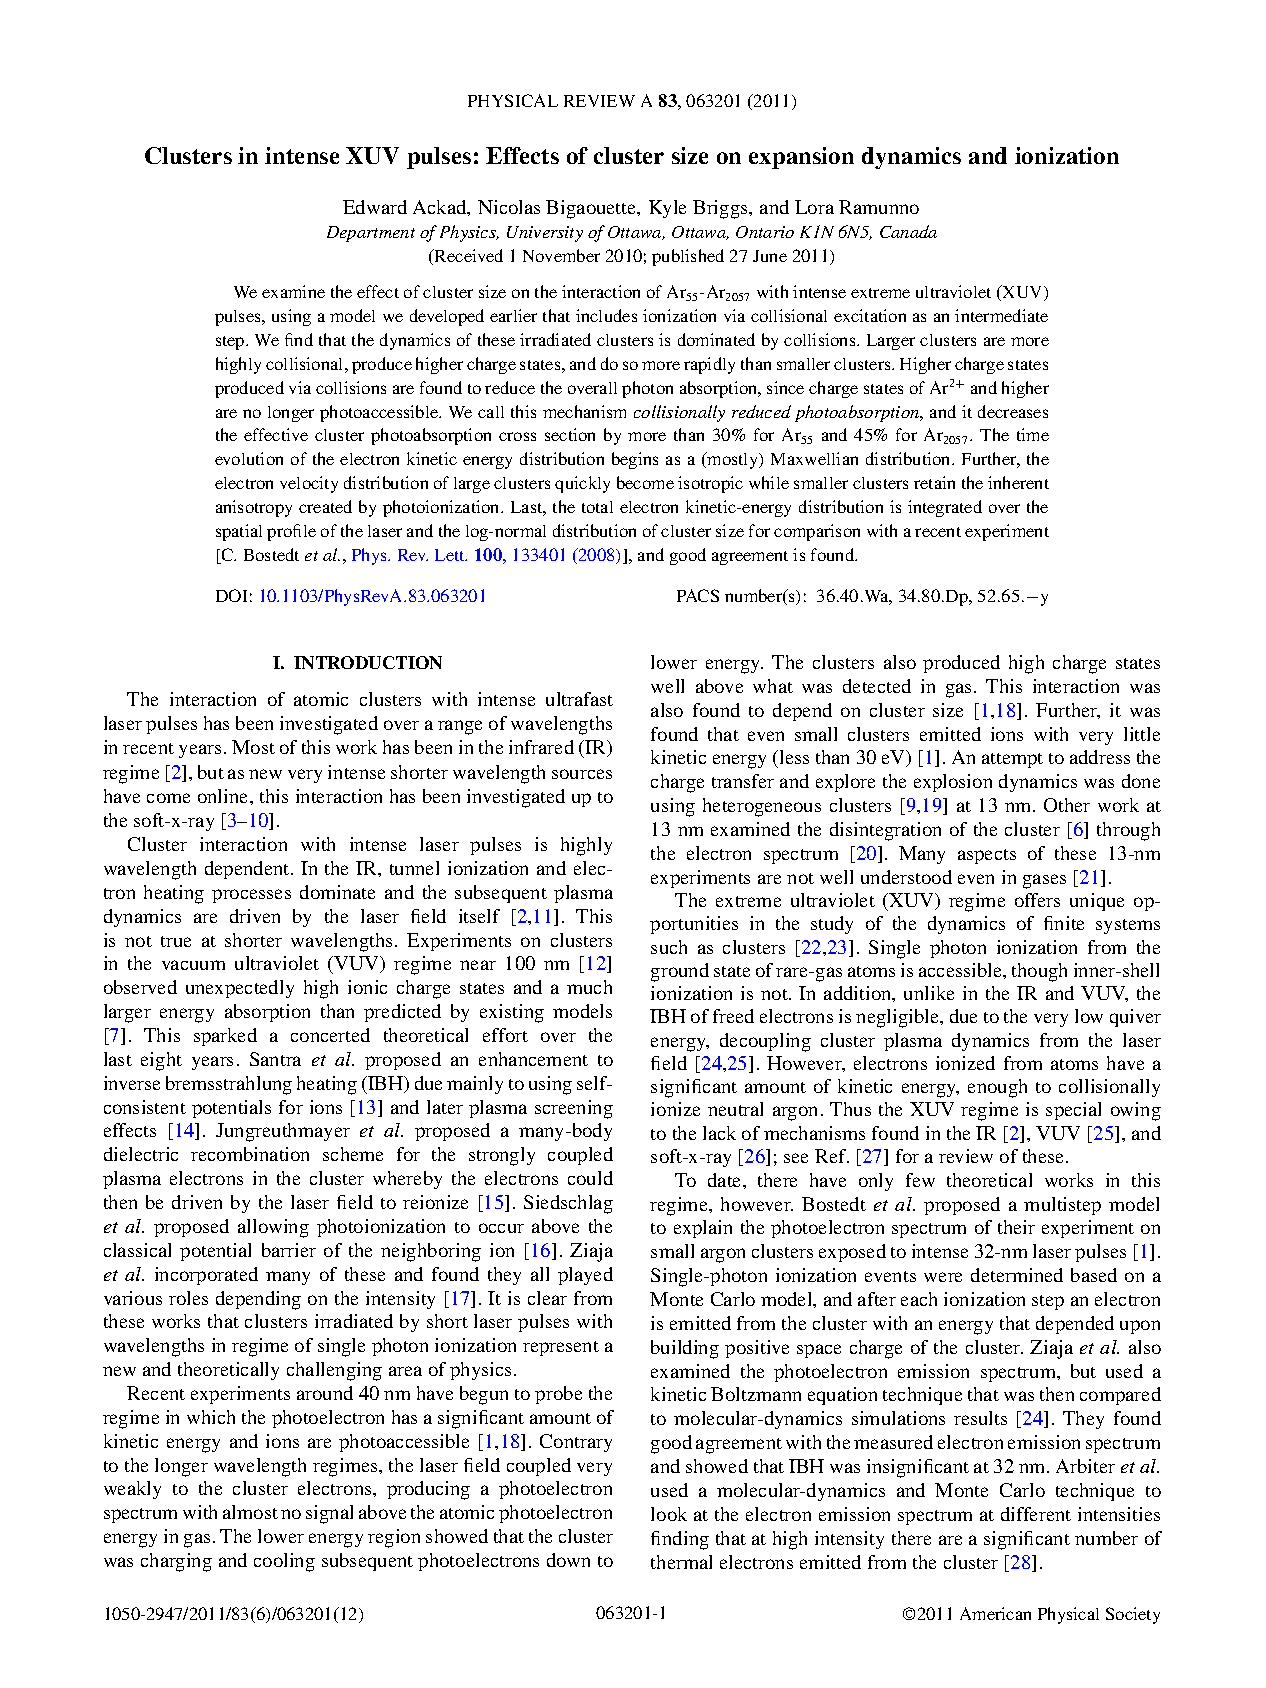
\includepdf[pages=-,
            addtotoc={
                %1,section,1,{\PaperTitleSize},paper_size,
                1,subsection,2,Introduction,paper_size_intro,
                2,subsection,2,Theory,paper_size_theory,
                3,subsection,2,Results,paper_size_results,
                3,subsubsection,3,Ions,paper_size_ions,
                3,paragraph,4,Charge state,paper_size_cs,
                3,paragraph,4,Charge state evolution,paper_size_cs_ev,
                5,paragraph,4,Excited states evolution,paper_size_es_ev,
                5,paragraph,4,Mechanisms of ionization,paper_size_ionization,
                6,paragraph,4,Charged shell structure,paper_size_shell,
                7,paragraph,4,Kinetic energy,paper_size_K,
                8,subsubsection,3,Electrons,paper_size_electrons,
                8,paragraph,4,Kinetic energy distribution,paper_size_distrib_K,
                9,paragraph,4,Velocity distribution,paper_size_distrib_v,
                10,paragraph,4,Connection with experiment,paper_size_exp,
                10,subsection,2,Summary,paper_size_summary,
                11,subsection,2,Acknowledgements,paper_size_ack,
                11,subsection,2,References,paper_size_ref
            }]{papers/Ackad2011b.pdf}


\newcommand{\PaperTitleACI}{Augmented collisional ionization via excited states in XUV cluster interactions}

\section{\PaperTitleACI}

\begin{flushright}
Edward Ackad, Nicolas Bigaouette, Lora Ramunno
\end{flushright}

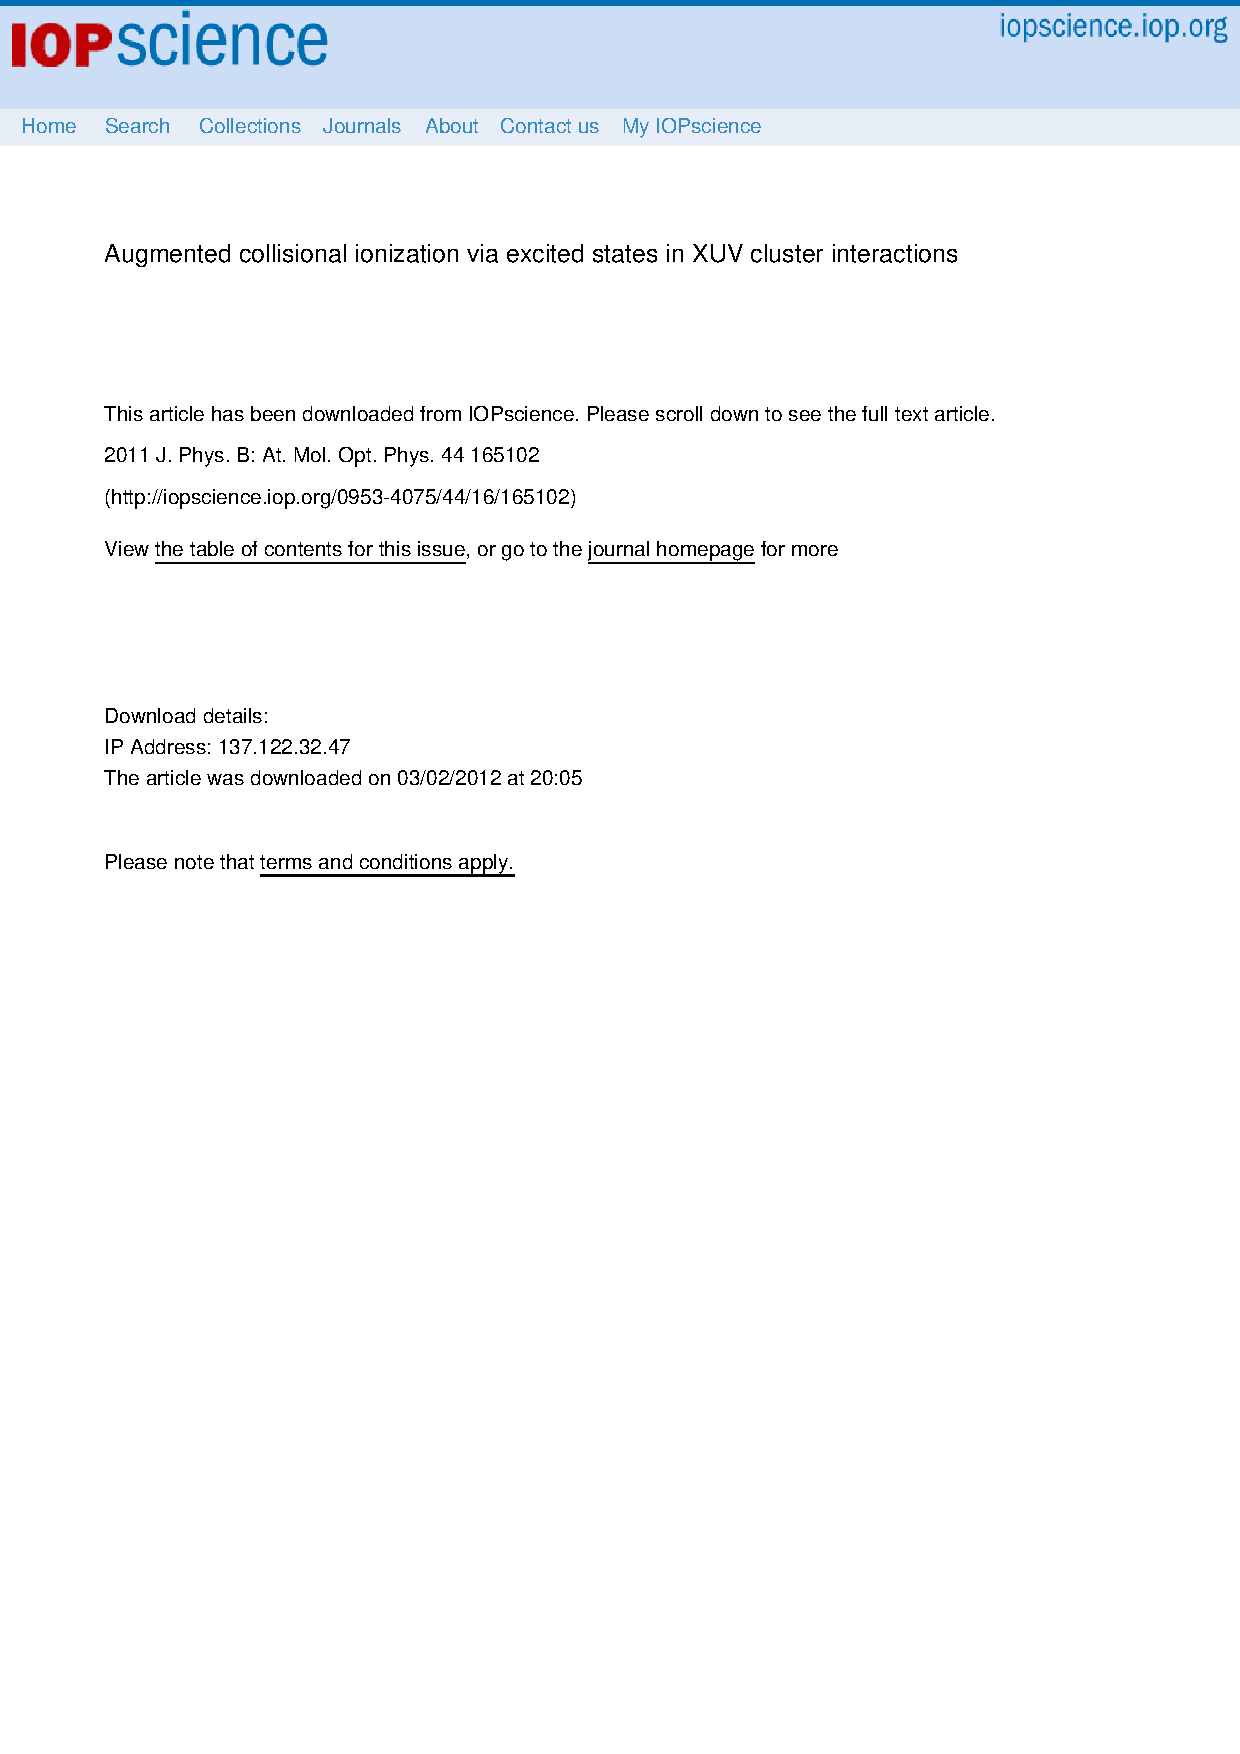
\includepdf[pages=2-,
            addtotoc={
                %2,section,1,{\PaperTitleACI},paper_aci,
                2,subsection,2,Abstract,paper_aci_abstract,
                2,subsection,2,Introduction,paper_aci_intro,
                3,subsection,2,Method,paper_aci_method,
                4,subsection,2,Results,paper_aci_results,
                6,subsection,2,Conclusion,paper_aci_conclusion,
                6,subsection,2,Acknowledgements,paper_aci_ack
            }]{papers/Ackad2011a.pdf}


\newcommand{\PaperTitleMapping}{Nonlinear grid mapping applied to an FDTD-based, multi-center 3D
                                  Schr\"odinger equation solver}

\section{\PaperTitleMapping}
\label{section:papers:qfdtd}

\begin{flushright}
Nicolas Bigaouette, Edward Ackad, Lora Ramunno
\end{flushright}


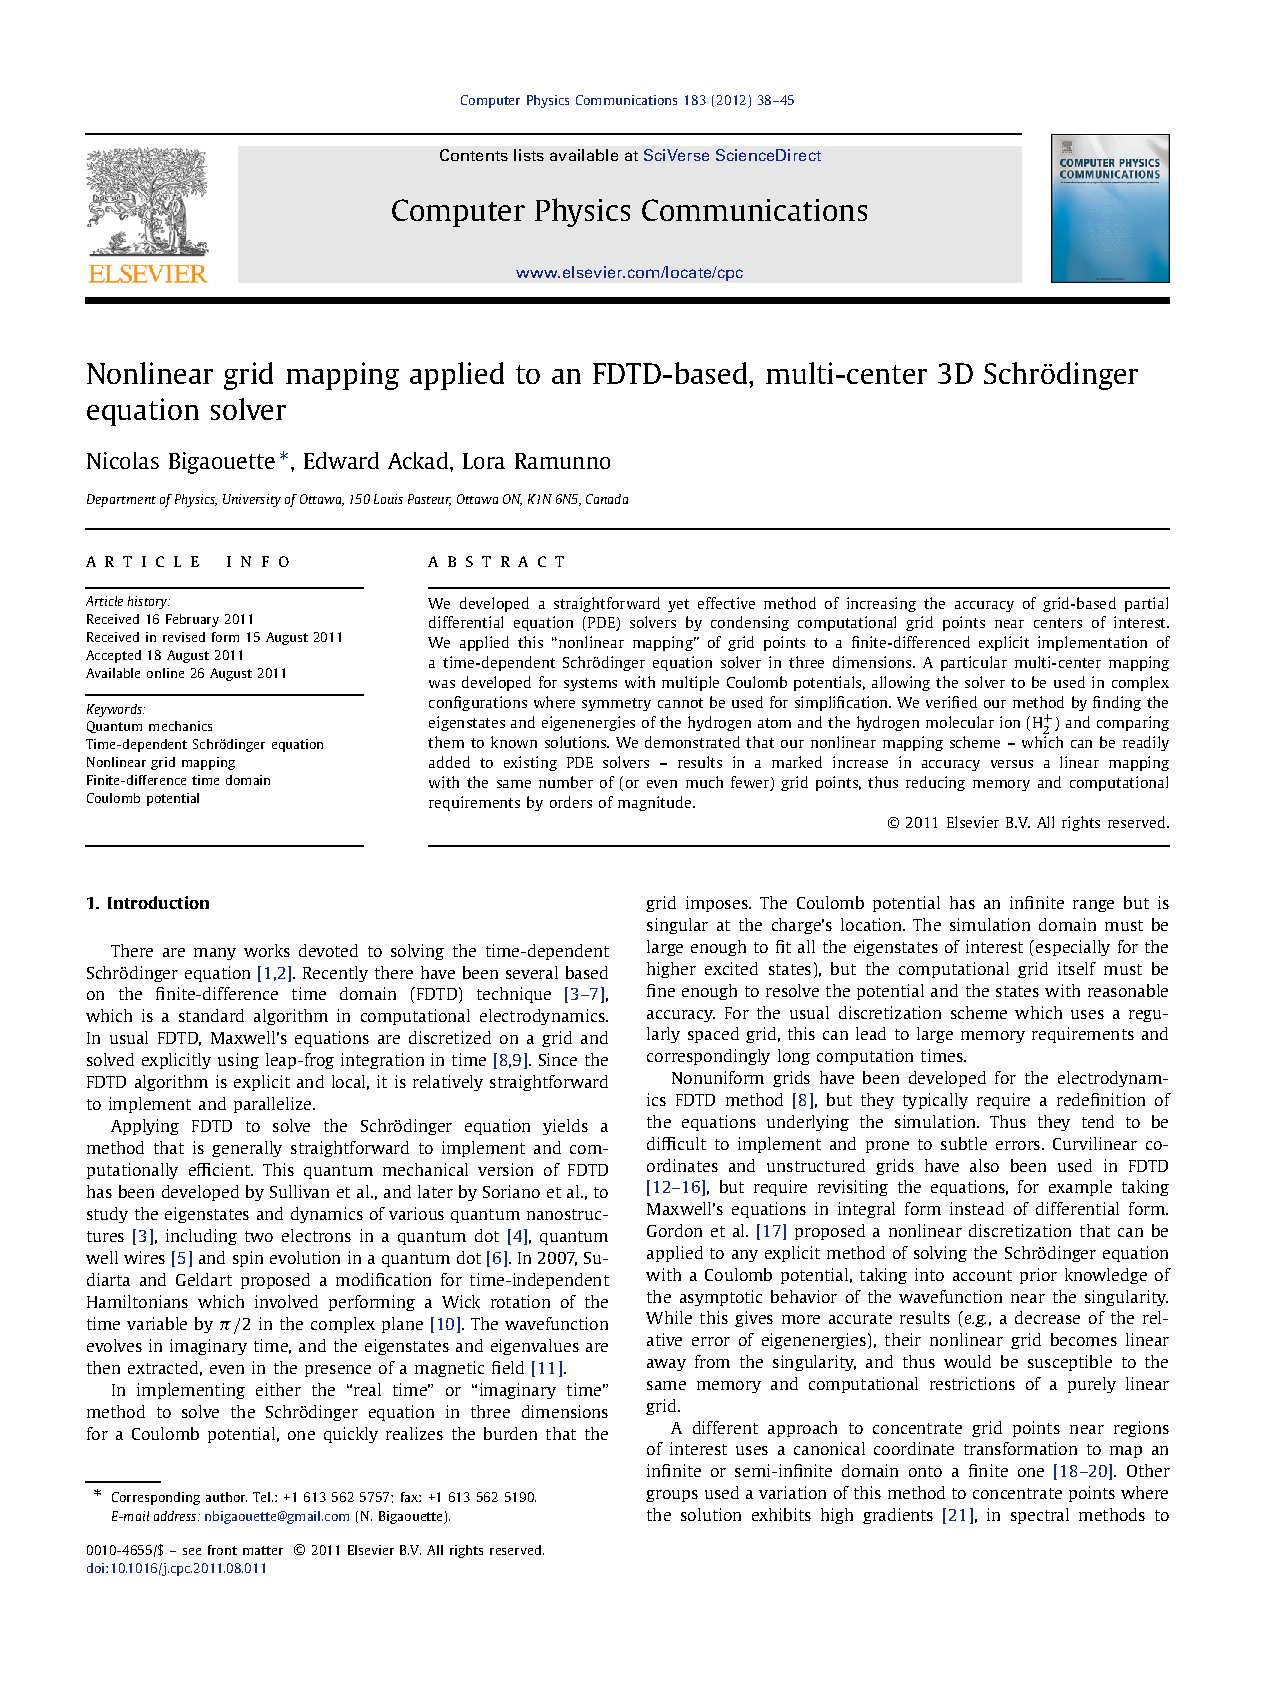
\includepdf[pages=-,
            addtotoc={
                %1,section,1,\PaperTitleMapping,paper_mapping,
                1,subsection,2,Abstract,paper_mapping_Abstract,
                1,subsection,2,Introduction,paper_mapping_intro,
                2,subsection,2,Finite-differenced Schrödinger equation,paper_mapping_fdtd,
                2,subsubsection,3,Real-time,paper_mapping_realtime,
                3,subsubsection,3,Imaginary-time,paper_mapping_imagtime,
                3,subsection,2,Details of nonlinear mapping,paper_mapping_details,
                4,subsubsection,3,General approach,paper_mapping_details_general,
                4,subsubsection,3,Details of the implementation,paper_mapping_details_details,
                5,subsubsection,3,Nonlinear mapping for the Coulomb potential,paper_mapping_details_coulomb,
                6,subsection,2,Validation and results,paper_mapping_results,
                6,subsubsection,3,Hydrogen atom,paper_mapping_results_h,
                7,subsubsection,3,Hydrogen cation molecule,paper_mapping_results_h2p,
                7,subsection,2,Conclusion,paper_mapping_conclusion,
                8,subsection,2,References,paper_mapping_ref
            }]{papers/Bigaouette2011_Mapping.pdf}


\section{Other contributions}

\lipsum[1]



\section{Conclusion}

Lorem ipsum dolor sit amet, consectetur adipiscing elit. Quisque accumsan commodo velit vitae varius. Aliquam dictum
vulputate gravida. Ut commodo, nulla in elementum feugiat, dolor lectus vehicula velit, eu accumsan dolor risus at nisi.
Mauris a leo nec urna consequat ornare. Etiam vitae quam vitae lectus lobortis sodales. Aenean sed nisi sit amet nulla
sagittis elementum. Duis lorem sem, varius eu mollis et, gravida sit amet risus. Nam luctus orci non dolor vehicula nec
adipiscing ante fringilla. Praesent porttitor hendrerit nulla, eget congue nibh auctor vel. Donec ac sem interdum tortor
interdum tristique. Morbi quis velit in erat ultricies fermentum. Nunc sit amet neque enim, sit amet hendrerit mi.




%\ReferencesSection{references}


\end{document}
